%\title{Using the forest package to create trees in LaTeX}
% From http://tex.stackexchange.com/a/108728/23931 
\documentclass[preview,border=0]{standalone}
\usepackage[paperheight=20cm,paperwidth=8cm]{geometry}
\usepackage{graphicx}
% \usepackage{forest}
\usepackage{amsmath}
\usepackage{tikz}
\usetikzlibrary{arrows,automata,positioning}


\begin{document} \begin{center}
		
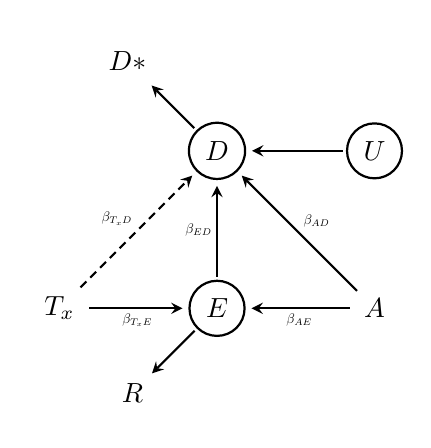
\begin{tikzpicture}[
	> = stealth, % arrow head style
	shorten > = 1pt, % don't touch arrow head to node
	auto,
	node distance = 2cm, % distance between nodes
	thick, % line style
	U/.style={circle, draw=black, outer sep=1.5pt, minimum size=3mm},  %draw=black, fill=white
	O/.style={circle, outer sep=-.8pt, minimum size=3mm},              %draw=white, fill=white
	]
	
	% Nodes and their relative positions
	\node[U] (D) {$D$};	
	\node[U] (U) [right of = D] {$U$};
	\node[U] (E) [below of = D] {$E$};
	\node[O] (R) [below left = .8 of E] {$R$};
	\node[O] (T) [left of = E] {$T_x$};
	\node[O] (A) [right of = E] {$A$};
	\node[O] (DD) [above left = .8 of D] {$D\ast$};
	
	% Paths connecting nodes
	\path[->] (T) edge[densely dashed] node[scale=0.5]{$\beta_{T_xD}$} (D);
	\path[->] (T) edge node[below,scale=0.5]{$\beta_{T_xE}$} (E);
	\path[->] (E) edge node[scale=0.5]{$\beta_{ED}$} (D);
	\path[->] (A) edge node[scale=0.5]{$\beta_{AE}$} (E);
	\path[->] (A) edge node[above right,scale=0.5]{$\beta_{AD}$} (D);
	\path[->] (D) edge (DD);
	\path[->] (U) edge (D);
	\path[->] (E) edge (R);

\end{tikzpicture}
	

\end{center}\end{document}
